\documentclass[12pt]{article}
\usepackage{graphicx}
\usepackage{caption}
\usepackage{setspace}
\setstretch{1.2}
\title{Is Florida Getting Warmer?}
\author{George Papaeracleous}
\date{26 October 2025}

\begin{document}
  \maketitle

  \section*{Results \& Interpretations}
  Observed Pearson correlation coefficient was calculated between year and temperature to be $r=0.53$ (Fig. 1).
  A permutation test, of 10,000 permutations, was done, and it gave a p-value of $p<0.01$, indicating a significant
  positive relationship between time and temperature (Fig.1 \& Fig.2). 

\begin{figure}[h!]
\centering
\begin{minipage}[b]{0.45\textwidth}
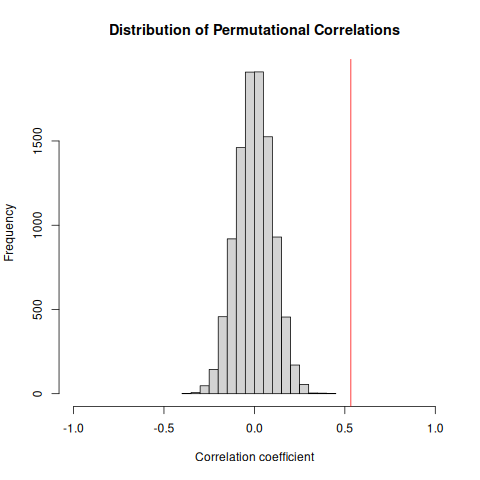
\includegraphics[width=\textwidth]{../results/florida_histogram.png}
\caption{Distribution of correlation coefficients from 10,000 permutations. Red line shows the observed correlation.}
\end{minipage}
\hfill
\begin{minipage}[b]{0.45\textwidth}
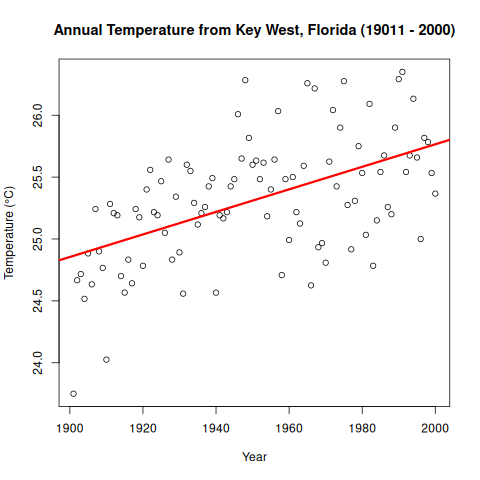
\includegraphics[width=\textwidth]{../results/florida_line_graph.png}
\caption{Annual mean temperature in Key West, Florida (1901–2000). Red line shows the linear trend.}
\end{minipage}
\end{figure}



\end{document}